\documentclass[11pt,a4paper,twoside,openright]{book}
\usepackage[utf8]{inputenc}
\usepackage[T1]{fontenc}
\usepackage{lipsum}% juste utile ici pour générer du faux texte}
\usepackage{mwe}%juste utile ici pour générer de fausses images
\usepackage{amsmath,amsfonts,amssymb}%extensions de l'ams pour les mathématiques
\usepackage{shorttoc}%pour la réalisation d'un sommaire
\usepackage{tikz}
\usepackage{tabularx,color,colortbl}
\definecolor{MPL1}{rgb}{0.89411765, 0.10196078, 0.10980392}
\definecolor{MPL2}{rgb}{0.21568627, 0.49411765, 0.72156863}
\definecolor{MPL3}{rgb}{0.30196078, 0.68627451, 0.29019608}
\definecolor{MPL4}{rgb}{0.59607843, 0.30588235, 0.63921569}
\usepackage{floatrow}
\usepackage{booktabs}
\usepackage{tikz}
\usepackage{tcolorbox}
\newcommand*\circled[1]{\tikz[baseline=(char.base)]{
\node[shape=circle,fill=orange!80!yellow,draw,inner sep=1pt,font=\bfseries] (char) {#1};}}
\floatsetup[table]{capposition=top}
\usepackage[first=0,last=9]{lcg}
\newcommand{\ra}{\rand0.\arabic{rand}}
\usepackage{graphicx}%pour insérer images et pdf entre autres
\graphicspath{{images/}}%pour spécifier le chemin d'accès aux images
\usepackage[left=2.5cm,right=1.5cm,top=2cm,bottom=2cm]{geometry}%réglages des marges du document selon vos préférences ou celles de votre établissement
\usepackage[Bjornstrup]{fncychap}%pour de jolis titres de chapitres voir la doc pour d'autres styles.
\usepackage{fancyhdr}%pour les en-têtes et pieds de pages
\setlength{\headheight}{14.2pt}% hauteur de l'en-tête

%%%%%%%%%%%%%%%%%%%style front%%%%%%%%%%%%%%%%%%%%%%%%%%%%%%%%%%%%%%%%% 
\fancypagestyle{front}{%
	\fancyhf{}%on vide les en-têtes
	\fancyfoot[C]{page \thepage}%
	\renewcommand{\headrulewidth}{0.4pt}%trait horizontal pour l'en-tête
	\renewcommand{\footrulewidth}{0.4pt}%trait horizontal pour les pieds de pages
}
%%%%%%%%%%%%%%%%%%%style main%%%%%%%%%%%%%%%%%%%%%%%%%%%%%%%%%%%%
\fancypagestyle{main}{%
	\fancyhf{}
	%\renewcommand{\CTV}{\fontfamily{phv}\selectfont\Huge \scshape}
	\renewcommand{\chaptermark}[1]{\markboth{\thechapter.\ ##1}{}}
	\renewcommand{\sectionmark}[1]{\markright{\thesection\ ##1}}
	\fancyhead[c]{}
	\fancyhead[RO,LE]{\rightmark}%
	\fancyhead[LO,RE]{}
	\fancyfoot[C]{}
	\fancyfoot[RO,LE]{page \thepage}%
	\fancyfoot[LO,RE]{\leftmark}
}
%%%%%%%%%%%%%%%%%%%style back%%%%%%%%%%%%%%%%%%%%%%%%%%%%%%%%%%%%%%%%%  
\fancypagestyle{back}{%
	\fancyhf{}%on vide les en-têtes
	\fancyfoot[C]{page \thepage}%
	\renewcommand{\headrulewidth}{0.4pt}%trait horizontal pour l'en-tête
	\renewcommand{\footrulewidth}{0.4pt}%trait horizontal pour les pieds de pages
}
%%%%%%%%%%%%%%%%%%%%%%%%%%%%index%%%%%%%%%%%%%%%%%%%%%%%%%%%%%%%%%%%%%%%
\usepackage{makeidx}
\makeindex
\usepackage[english]{babel}%pour un document en français
\usepackage{listings}%pour insérer du code source
\usepackage{hyperref}%rend actif les liens, références croisées, toc…
\hypersetup{colorlinks,%
	citecolor=black,%
	filecolor=black,%
	linkcolor=black,%
	urlcolor=black} 
%%%%%%%%%%%%%%%%%%%%%%%%%%%%biblio%%%%%%%%%%%%%%%%%%%%%%%%%%%%%%%%%%%%%%
\usepackage[style=chem-acs,sorting=none,backend=bibtex]{biblatex}
\AtEveryBibitem{%
	\clearfield{note}%
}
\addbibresource{references/refs.bib}% pour indiquer où se trouve notre .bib
\usepackage{csquotes}% pour la gestion des guillemets français.
%%%%%%%%%%%%%%%%%%%%%%%%%%%%%glossaire%%%%%%%%%%%%%%%%%%%%%%%%%%%%%%%%%%%
\usepackage{glossaries}
\makeglossaries         

\makeatletter
\newenvironment{abstract}{%
	\cleardoublepage
	\null\vfil
	\@beginparpenalty\@lowpenalty
	\begin{center}%
		\bfseries \abstractname
		\@endparpenalty\@M
\end{center}}%
{\par\vfil\null}
\makeatother
%%%%%%%%%%%%%%%%%%%%%%%%%%%%%%%%%%%%%%%%%%%%%%%%%%%%%%%%%%%%%%%%%%%%%%%%%%
\newcommand{\fig}[3]{\begin{figure}[h!]
	\centering
	\includegraphics[width = #2\linewidth]{#1}
	\caption{#3}
\end{figure}}

\usepackage{xcolor}
\newcommand{\red}[1]{{\color{red}#1}}
\newcommand{\blue}[1]{{\color{blue}#1}}
\newcommand{\green}[1]{{\color{green}#1}}

\newcommand{\black}[1]{{\color{black}#1}}

\newcommand{\vv}[1]{\vec{#1}}

% fancy verbatim :
\usepackage{fancyvrb}
\newcommand{\vrb}[1]{\begin{Verbatim}[commandchars=\\\{\}]
#1
\end{Verbatim}}
\usepackage{multirow}
\usepackage{array}
\usepackage{hyperref}
%% works with `url` only as well:
%\usepackage{url}

\usepackage{xcolor}
\usepackage[normalem]{ulem}
\useunder{\uline}{\ulined}{}%
\DeclareUrlCommand{\bulurl}{\def\UrlFont{\ttfamily\color{blue}\ulined}}
\newcolumntype{C}{>{\centering\arraybackslash}p{2.5cm}}
\usepackage{tikz}
\usetikzlibrary{shapes.geometric, arrows}
\usetikzlibrary{shapes.multipart}
\tikzstyle{startstop} = [rectangle, rounded corners, minimum width=3cm, minimum height=1cm,text centered, draw=black, fill=red!30]
\tikzstyle{startstop2} = [rectangle, rounded corners, minimum width=3cm, minimum height=1.5cm,text centered, draw=black, fill=orange!30,ultra thick]
\tikzstyle{decision} = [diamond, minimum width=3cm, minimum height=1cm, text centered, draw=black, fill=green!30]
\tikzstyle{decision2} = [diamond, minimum width=3cm, minimum height=1cm, text centered, draw=black, fill=blue!30,ultra thick]
\tikzstyle{arrow} = [thick,->,>=stealth]
\tikzstyle{arrowT} = [ultra thick,->,>=stealth]

\begin{document}
	\frontmatter% début des pages liminaires
	\pagestyle{front}%style des en-têtes pour cette partie
	\begin{titlepage}
	\parindent=0pt
	\bfseries\Large Master 2 Physics Photonics Nanotechnology \hspace*{\stretch{1}} 2022-2023
	\vspace{1cm}
	
	\begin{center}
		
\includegraphics[height=3cm]{images/logo_ub.png}%
		\hfill
		
\includegraphics[height=4cm]{images/logo_ubfc.png}%
	\end{center}
	\vspace{1cm}
	\hrulefill
	
	\begin{center}
		\bfseries\huge
		Functional modes and thermal B-factor predictions for multigenic structural analysis predicted from Alpha Fold
	\end{center}
	\hrulefill
	\vspace{.5cm}
	
	\begin{center}
		\bfseries\Large
		Nicolas PETIOT
	\end{center}
	
	\begin{center}
		\normalfont \today
	\end{center}
	\vspace{.25cm}
	
	\begin{center}
		\bfseries\Large
		\underline{Supervisors}: Dr. Adrien NICOLAÏ and Pr. Patrick SENET
	\end{center}
	\vspace{.25cm}
	
	\begin{center}
		\bfseries\Large
		NANOSCIENCES Department - Physics Applied to Proteins
	\end{center}
	\vspace{.25cm}
	
	\begin{center}
		\normalfont \large Laboratoire Interdisciplinaire Carnot de Bourgogne, UMR 6303 CNRS\\
	Université de Bourgogne Franche-Comté / Faculté des Sciences et Techniques Mirande\\
	9, Av. Savary - B.P. 47 870 21078. DIJON CEDEX - France
	\end{center}	

	\vspace{.5cm}

	
\includegraphics[height=2cm]{images/logo_icb.png}
	\hfill
	
\includegraphics[height=2cm]{images/logo_cnrs.png}
	\hfill 
	
\includegraphics[height=2cm]{images/logo_eiphi.png}
	\hfill
	
\includegraphics[height=2cm]{images/logo_investir.png}
	\vspace{.5cm}
	\begin{center}
		
\includegraphics[height=2cm]{images/logo_rbfc.png}
		\hspace{2cm}
		
\includegraphics[height=2cm]{images/logo_feder.png}
	\end{center}
	
\end{titlepage}%on crée la couverture
	\thispagestyle{empty}%pour la page de garde toute blanche
	\thispagestyle{empty}% pour une page sans en-tête ni pieds de page
%\chapter*{Résumés}
\addcontentsline{toc}{chapter}{Abstract}%Pour l'ajout dans la table des matières au même rang que chapitre
\begin{abstract}
%Proteins are complex biomolecules that are critical to the functioning of living organisms. They are made up of sequences of amino-acids that fold into specific three-dimentional structures, which is highly related to their function. The process of protein folding is considered one of the most challenging problems in the field of biology and biochemistry, as it involves a delicate interplay of chemical and physical forces that determine the final shape of the protein. AlphaFold is a groundbreaking tool developped by DeepMind that uses artificial intelligence algorithms to pedict 3D structure of proteins based on their amino-acid sequence. This tool has the potential to revolutionize the study of enzymes as it provides fast and accurate way to predict the structure of molecules that have catalytic properties. The present work aim at using AlphaFold to study the catalytic properties of Glutathione Transferase (GST), especially from class $\delta$ and $\varepsilon$ of \textit{drosophilia melanogaster}, whith the ultimate goal of being able to design brand new sequences for enzymes with improved catalytic efficiancy.\\
%\noindent In addition to using AlphaFold for the generation of 3D structures, molecular dynamics simulations can also be performed based on these structures. It allows to predict some of their potential behaviour and study various factors that may influence the function of the protein, such as thermal fluctuations or protein-ligand interactions. Simulationg these processes gives a deeper understanding of how proteins function and allows to identify areas for further investigation and improvements. 
	  
\end{abstract}
\thispagestyle{empty}%%no comment !
	\thispagestyle{empty}% pour une page sans en-tête ni pieds de page
%\chapter*{Résumés}
\addcontentsline{toc}{chapter}{Acknowledgements}%Pour l'ajout dans la table des matières au même rang que chapitre
\renewcommand{\abstractname}{Acknowledgements}
\begin{abstract}
text here
\end{abstract}
%no comment !
	\tableofcontents
	%
	\mainmatter% corps du document
	\pagestyle{main}%style des en-têtes pour cette partie
	\chapter{Introduction}
Proteins are biological macromolecules that perform a large variety of functions in living cells comprising biochemical (enzymes), structural, mechanical, and signaling functions. They consist of chains composed of 20 different amino-acids. To perform their functions, proteins interact with small molecules referred to as ligands, which are able to bind to a protein with high affinity and specificity \cite{du2016insights}. These protein/ligand interactions are crucial in biology, particularly in the context of drug design \cite{li2019predicting}. Since proteins interact with a broad range of drugs, it is of particular interest to study the mechanisms of binding of ligands to proteins and its impact on the structural dynamics to gain insights into (i) phenomena involved in the biological process and related to diseases \cite{silva2010ligand} (misfolding, aggregation), and (ii) discovery, design, and development of new drugs \cite{payandeh2021ligand}. The experimental structural data (e.g., X-ray crystallography, NMR, or cryo-EM) provide key structural information of the ligand-bound and ligand-unbound (APO) proteins \cite{chakraborti2021all}. Nevertheless, the static information is not always sufficient for understanding protein–ligand binding mechanisms, especially when pockets are highly flexible and contain several binding sites. Therefore, molecular dynamics (MD) and Normal Mode Analysis (NMA) are powerfull tools that provides a description of the dynamics and structures of protein–ligand systems with a high spatial and temporal resolution.
\section{Glutathione Transferase}
Glutathione transferases (GSTs) belong to a ubiquitous superfamily of enzymes that
metabolize a broad range of reactive toxic compounds by catalyzing the conjugation of reduced tripeptide glutathione ($\gamma$-Glu-Cys-Gly; named GSH) to the electrophilic center of a second substrate \cite{mannervik1985isoenzymes, armstrong1997structure, hayes2005glutathione}, the reactivity of GSH being due to the thiol group SH of the cysteine residue. The conjugation reaction occurs spontaneously but GST accelerates it dramatically. This process of detoxification protects cells against damages caused by both exogenous and endogenous molecules. GSTs were first discovered in liver cells \cite{combes1961liver}, and since then, they have been found to exhibit ligand-binding properties for a large variety of compounds, which are not always their enzymatic substrates \cite{axarli2004characterization}. Therefore, GSTs participate in diverse biological processes, making them multifunctional proteins. Moreover, GSTs are classified into three families according to their location in the cell: cytosolic, mitochondrial, and microsomal, which is not evolutively related to the two other classes \cite{oakley2011glutathione}. First-discovered and most-abundant cytosolic GSTs are divided into 13 classes based on homology of their sequences.Members of the same cytosolic class have at least $40\%$ of sequence identity, while members of different classes must have at most $25\%$ of sequence identity. Even if they present a low homology with the cytosolic GST, mitochondrial GSTs can be considered as a particular class of GSTs (Kappa). Among the 42 GSTs identified in \textit{Drosophila melanogaster}, $\delta$ and $\varepsilon$ are the largest classes, with 25 members \cite{F-Neiers-GSTs}. In their catalytic cycle, the GSH usually binds in a specific set of amino-acids called G-site and the hydrophobic xenobiotic in the so-called H-site. Interactions between insects and plant’s chemicals lead to a major driving force in herbivorous insect evolution, hence this encourages the study of insect GSTs to understand how spontaneous mutations modify the stability, selectivity and the catalytic efficiencies of this enzyme superfamily.
% figure 1 : catalytic cycle of GSTs + evolutionary relationship between GSTs (F. Neiers)
\section{AlphaFold}
X-ray diffraction is a powerful experimental technique that have been used extensively to determine the three-dimentional structures of proteins. 
% cite XRD ?
In this technique, a crystal of the protein is bombarded with X-rays, and the resulting diffraction pattern is used to determine the position of atoms within the protein. Over the years, X-ray diffraction experiments have played a pivotal role in determining the structures of tens of thousand of proteins, which are deposited in the Protein Data Bank (PDB). 
% cite PDB ?
However, this experimental process can be time-consuming and technically challenging. Moreover, compared to the vast number of known protein sequences, the ensemble of solved structure is insignificant. In 2021, DeepMind \cite{AlphaFold} used machine learning approaches with the AlphaFold program. It uses computational models to predict the 3D structures of proteins based on it amino-acid's sequence with a high accuracy. In the field of de novo design of enzymes, AlphaFold has the potential to revolutionize the way we consider the design process, allowing to predict 3D structures that have not yet been experimentally characterized.\\
\noindent In addition to the initial AlphaFold program, DeepMind developped several other tools that have further expanded the capacities of protein structure predictions. One such tool is AlphaFold-multimer\cite{Multimer}, which allows predictions for the structure of protein complexe such as homodimers. An other one is AlphaFill\cite{AlphaFill}, which predict the positions of ligands, small molecules that bind to protein such as Glutathione. All together, these tools represent a major step forward in the field of protein study and will be at the root of the present work.
\section{Goals}

	\chapter{Materials and Methods}
\section{Multiple Sequence Alignment}
Multiple sequence alignment (MSA) is a fundamental technique in bioinformatics used to compare and analyze the similarities and differences between multiple biological sequences. These sequences can be DNA, RNA, or protein sequences and can come from various species or different regions of the same genome. By aligning these sequences, it is possible to identify conserved regions that are important for function or evolution, as well as unique features that differentiate the sequences.
% add picture from F. Neiers ?
In this study, we focus on a set of 25 GSTs sequences related to each other through evolution. Each sequence has a different length, making the alignment process especially useful. Through this analysis, we aim to identify regions of conservation and divergence between the sequences (see exemple below). Our first task was to use MSA to predict both the position of the interface of dimerization and the binding site of the set of GST sequence. The stability of the dimer structure is dependent on the interactions at this interface. Therefore, understanding the location and conservation of the dimer interface can provide insights into the stability of the dimer structure and the mechanisms of the biological activity. On the other hand, the binding site is the specific location on the enzyme where a substrate or ligand binds and interacts. The catalytic efficiency of the enzyme is related to the binding site because it determines the specificity and strength of the substrate-enzyme interaction. Therefore, understanding the location and conservation of the binding site is essential for elucidating the function and mechanism of action of the enzyme.\\
\\
\noindent Each cell in the MSA matrix corresponds to a particular amino acid at a particular position in a particular sequence. We refer to the position in the MSA matrix as the MSA index. The MSA index allows us to compare the amino acid residues at each position across all the sequences in the alignment. We focused on highlighting residues that are known to be part of the dimer interface or binding site. By doing so, we can compare these residues across all sequences and identify any conserved or variable regions.

\begin{figure}
	\label{MSA sample}
	\begin{verbatim}
          GSTD1  SPC-RSVIMTAKAVGVELNKKLLNLQAGEHLKPEFLKINPQHTIPTLVDNGFALWESRAI
          GSTE1  SPCVRTVKLTLKVLNLDYEYKEVNLQAGEHLSEEYVKKNPQHTVPMLDDNGTFIWDSHAI
                 SPC R+V +T K + ++   K +NLQAGEHL  E++K NPQHT+P L DNG  +W+S AI
	\end{verbatim}	
	\caption{Sample of a multiple sequence alignment. In such matrix, gaps are represented with the symbol "-". If a residue is conserved, it apears in the last row of the alignment, the residues are in a identical chemical class, thelast raw contains the symbol "+" and eventually, two very different residues are represented by an empty space.}
\end{figure}
\section{Anisotropic Network Model}
As seen in the introduction, the AlphaFold program allows for the prediction of protein structures with remarkable accuracy. These structures have the potential to be used in a wide range of applications, including molecular dynamics simulations. In this work, we aim to use AlphaFold-predicted structures as input for the Anisotropic Network Model (ANM) to study protein dynamics. Specifically, we will compare the results obtained from the ANM simulations using AlphaFold structures with those obtained using experimentally determined structures. More precisely, we will use the ANM to predict the thermal B-factors of the studied structures\cite{ANM-COM}, which are important indicators of protein flexibility and stability. The insights gained from this study will contribute to the ongoing efforts to develop computational tools for protein structure analysis and facilitate a deeper understanding of protein dynamics and function. To achieve these goals, it is necessary to provide a detailed description of the ANM and its underlying mathematical principles. The ANM is a widely used method for studying the collective motions and dynamics of proteins based on their structure. It models the protein as a network of connected nodes and springs (representing covalent and non-covalent interactions between them). 

\subsection{Theory}
\noindent Let $\vv{r_i}$ being the position of the node $i$ and $M_i$ it's mass. In the ANM, each node is assumed to be at the bottom of an harmonic potential, since interactions are modeled by connections between nodes, the force matrix is obtained by computing the mass-weighted Hessian matrix
\begin{equation}
	\label{mass-weighted hessian matrix}
	\hat{H}_{ij} = -\frac{\Gamma_{ij}\gamma}{\sqrt{M_iM_j}}\cfrac{\vv{R_{ij}}\vv{R}^T_ {ij}}{R^2_ {ij}}
\end{equation}
where $\gamma$ is the spring constant used to model interactions between nodes, $\vv{R}_{ij} = \vv{R}_j - \vv{R}_i$ and $\Gamma$ is the contact matrix. In the case were $i = j$, the force matrix is computed so that the self interacting term is the response to all the applied forces.
\begin{equation}
	\label{self interacting terms}
	\hat{H}_{ii} = -\sum_{j \ne i}\hat{H}_{ij}
\end{equation}
$\Gamma_{ij}$ is the contact matrix that allow or not two nodes to be interacting with each other. The normal modes and eigenfrequencies are given by the diagonalization of the mass-weighted Hessian matrix.
\begin{equation}
	\label{eigen equation}
	\hat{H}\vv{e}_k = \tilde{\omega}_k^2\vv{e}_k
\end{equation}
It is important to make some remarks at this point, first in the equation (\ref{mass-weighted hessian matrix}) $\hat{H}_{ij}$ is actually a three by three matrix. It means that the ovearall $\hat{H}$ will be a square matrix of dimention $d = 3N$ with $N$ the number of considered nodes. Since the diagonalization algorythms have a complexity of $O(d^3)$, it means that the computation time will highly depends on the choosen set of nodes. Second, the masses of the nodes are expressed in g.mol$^{-1}$ to avoid numerical errors in the diagonalization. Expressing $\gamma$ in kcal.mol$^{-1}$.\AA$^{-2}$, it means that the eigenvalues $\tilde{\omega}_k^2$ are expressed in kcal.g$^{-1}$.\AA$^{-2}$ which is directly proportional to a squared frequency $\omega^2 = 4.184 \times 10^{26}$ s$^{-2}$. Thermal B-factors of the node $i$ is directly proportionel to the mean squared fluctuations of the node's position $\sigma^2(\vv{R_i})$ and can be computed from the normal modes using the following 
\begin{equation}
	\label{thermal B-factors}
	\beta_i = \frac{8\pi^2}{3}\frac{k_BT}{M_i}\sum_k\cfrac{\vert\vv{e}_{k, i}\vert^2}{\tilde{\omega}_k^2}
\end{equation}
where $\vv{e}_{k, i}$ contains the elements of $\vv{e}_k$ related to the node $i$. $\beta_i$ is expressed in $m^2$ but will always be converted in $\AA^2$ because of conventions and usual order of magnitude.\\
\noindent Ever since the beginning, we were talking in a very abstract way about "nodes". In this work, we did consider the amino-acid's center of mass (COM). When available, we compared the predicted values of B-factors with X-ray based measurement in term of pearson correlation.
\begin{equation}
	\label{pearsonr}
	\mathcal{R} = \cfrac{\displaystyle\sum_i (\beta_i - <\beta>_i)(B_i - <B>_i)}{\sqrt{\displaystyle\sum_i(\beta_i - <\beta>_i)^2}\sqrt{\displaystyle\sum_j(B_j - <B>_j)^2}}
\end{equation}
The values of $\mathcal{R}$ are between $-1$ and $1$ and gives the linear correlation between predicted and measured B-factors. A coefficient of $1$ is associated to a perfect correlation wherease a coefficient of $0$ means that there is basically no links between prediction and experiment. Eventually, a negative value of $\mathcal{R}$ means that there is a correlation with opposite sign and would be interpreted as a result even worst than no correlation. Note that we need to consider the same ensemble of points for $\beta_i$ and $B_i$.\\
\noindent The thermal fluctuation of the nodes is not the only informations one can get from normal modes, indeed fluctuations of the $\vv{R}_{ij}$ vector can also be an interesting metric to analyse as it represents the relative motion of nodes within a given mode. 
\begin{equation}
	\label{metric dij}
	d_{ij} = k_BT\sum_k \frac{1}{\omega_k^2}\left( \frac{\vv{e}_{k, j}}{\sqrt{M_j}} - \frac{\vv{e}_{k, i}}{\sqrt{M_i}} \right)^2
\end{equation}
Such metric is especially interesting to study as it provide insights about the fluctuations of a mode with respect to another and allow to identify pairs of nodes involved in specific functional modes.
\subsection{Parametrization}
In the Anisortopic network model as presented above, we consider two parameters namely the contact matrix $\Gamma_{ij}$ and the spring constant $\gamma$. In order to get predictions that are physically relevant, it is necessary to compute the good parameters. Let us first consider the contact matrix. Given two nodes $i$ and $j$, we will consider $\Gamma_{ij} = 1$ if the distance $\vert\vv{R}_{ij}\vert$ is smaller than the cut-off $R_c$. It is then necessary to find a good numerical value for $R_c$. We know that for high distances, the interactions between the nodes are supposed to be small if not nulls. To add this kind of interactions, we look for $R_c$ as small as possible. We also know that the eigenvalues are associated to frequencies for the collectives modes. The six firsts modes should be global transations and rotations with a null frequency associated. In the case where $R_c$ is too small, some other modes will have null eigenfrequencies with no physical justifications. $R_c$ is then the smallest value that gives exactly $6$ null eigenvalues for the Hessian. Eventually, in the equation (\ref{mass-weighted hessian matrix}) $\gamma$ is a constant, it means that $\tilde{\omega}_k^2 \propto \gamma$. From the equation (\ref{thermal B-factors}), one can show that $\beta_i$ is inversly proportional to $\gamma$ which is just a scaling factor. It can then be computed from comparitions with experimental measurments of thermal B-factors using least squared methods.

\section{Molecular Dynamics}
Molecular dynamics (MD) has emerged as a powerful computational tool for simulating molecular systems with exceptional precision. By numerically integrating the equations of motion for atoms and molecules, MD provides detailed information about the dynamic behavior and interactions within these systems. With its ability to capture the atomic-level motion and thermodynamics, MD offers insights into the structural changes, energetics, and properties of molecules under various conditions. Compared with ANM, MD stands out for its superior precision in capturing the dynamic behavior of molecular systems. For the purpose of this work, the amount of system to be studied is far too big ($25$ structures $\times 3$ states in the catalytic cycle) and cannot be considered as an option. But considering it's accuracy, one can consider a sample of GSTs that will be simulated via MD.\\
MD consider interactions between atoms in a large variety of form. First, non-bonded interactions are considered with a lehnard-jones potential and electrostatic interactions.
\begin{equation}
	\label{non-bonded}
	V_{\text{non-bonded}}(\vv{r}_i) = \sum_j 4\epsilon_{ij}\left[ \left( \frac{\sigma_{ij}}{R_{ij}} \right)^{12} - \left( \frac{\sigma_{ij}}{R_{ij}} \right)^{6} \right] + \sum_j\cfrac{q_iq_j}{4\pi\epsilon_0R_{ij}}
\end{equation}
Interactions between bonded atoms are also described by the following.
\begin{equation}
	\label{bonded}
	V_{\text{bonded}}(\vv{r}_i) = \sum_{\text{bonds}} K_l(l - l_0)^2 + \sum_{\text{angles}} K_\theta(\theta - \theta_0)^2 + \sum_{\text{tortions}} K_\varphi [1 + \cos (n\varphi + \delta)]
\end{equation}
The ensemble of parameters for those interactions are optimized and used by MD algorithms by the so called force fields. Since the potential consider interactions between all the atoms of the system, this kind of simulation is called All Atoms MD, in opposition to coarse grained MD that we wont discuss here. Finally forces of interactions are obtained taking the gradient of the potential and the simulation is achieved by integration of the Newton's equation :
\begin{equation}
	\label{Newton}
	m\frac{d^2\vv{r}_i}{dt^2} = -\vv{\nabla}V(\vv{r}_i)
\end{equation}
From the time serie obtained, one can compute the associated Thermal B-Factors as mean squared fluctuations of the atom's position.
\begin{equation}
	\label{MD thermal B-factors}
	\beta_i = \frac{8\pi^2}{3}\left(\left< \vv{R}_i^2 \right> - \left< \vv{R}_i \right>^2\right)
\end{equation}
Comparisons between such factors computed from MD and from ANM gives again extra informations about the precision of the considered models.
	\chapter{Results and Discussion}

\section{Sequences and Static Structures}

\begin{figure}[h!]
	\label{Sequence & Structure}
	%\raggedright\textbf{A}
	%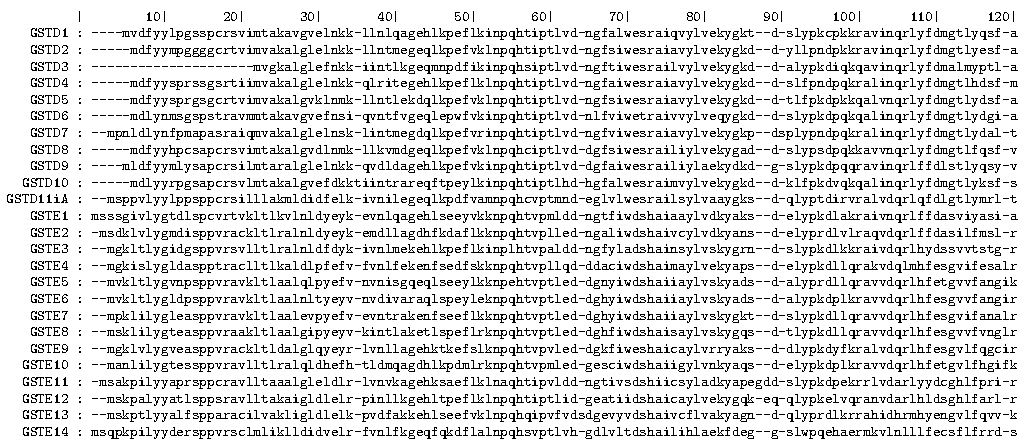
\includegraphics[width = .99\linewidth]{figures/MSA_1-120_empty.pdf}\\[.5cm] % MSA
	\begin{minipage}{.32\linewidth}
		\textbf{A}\\
		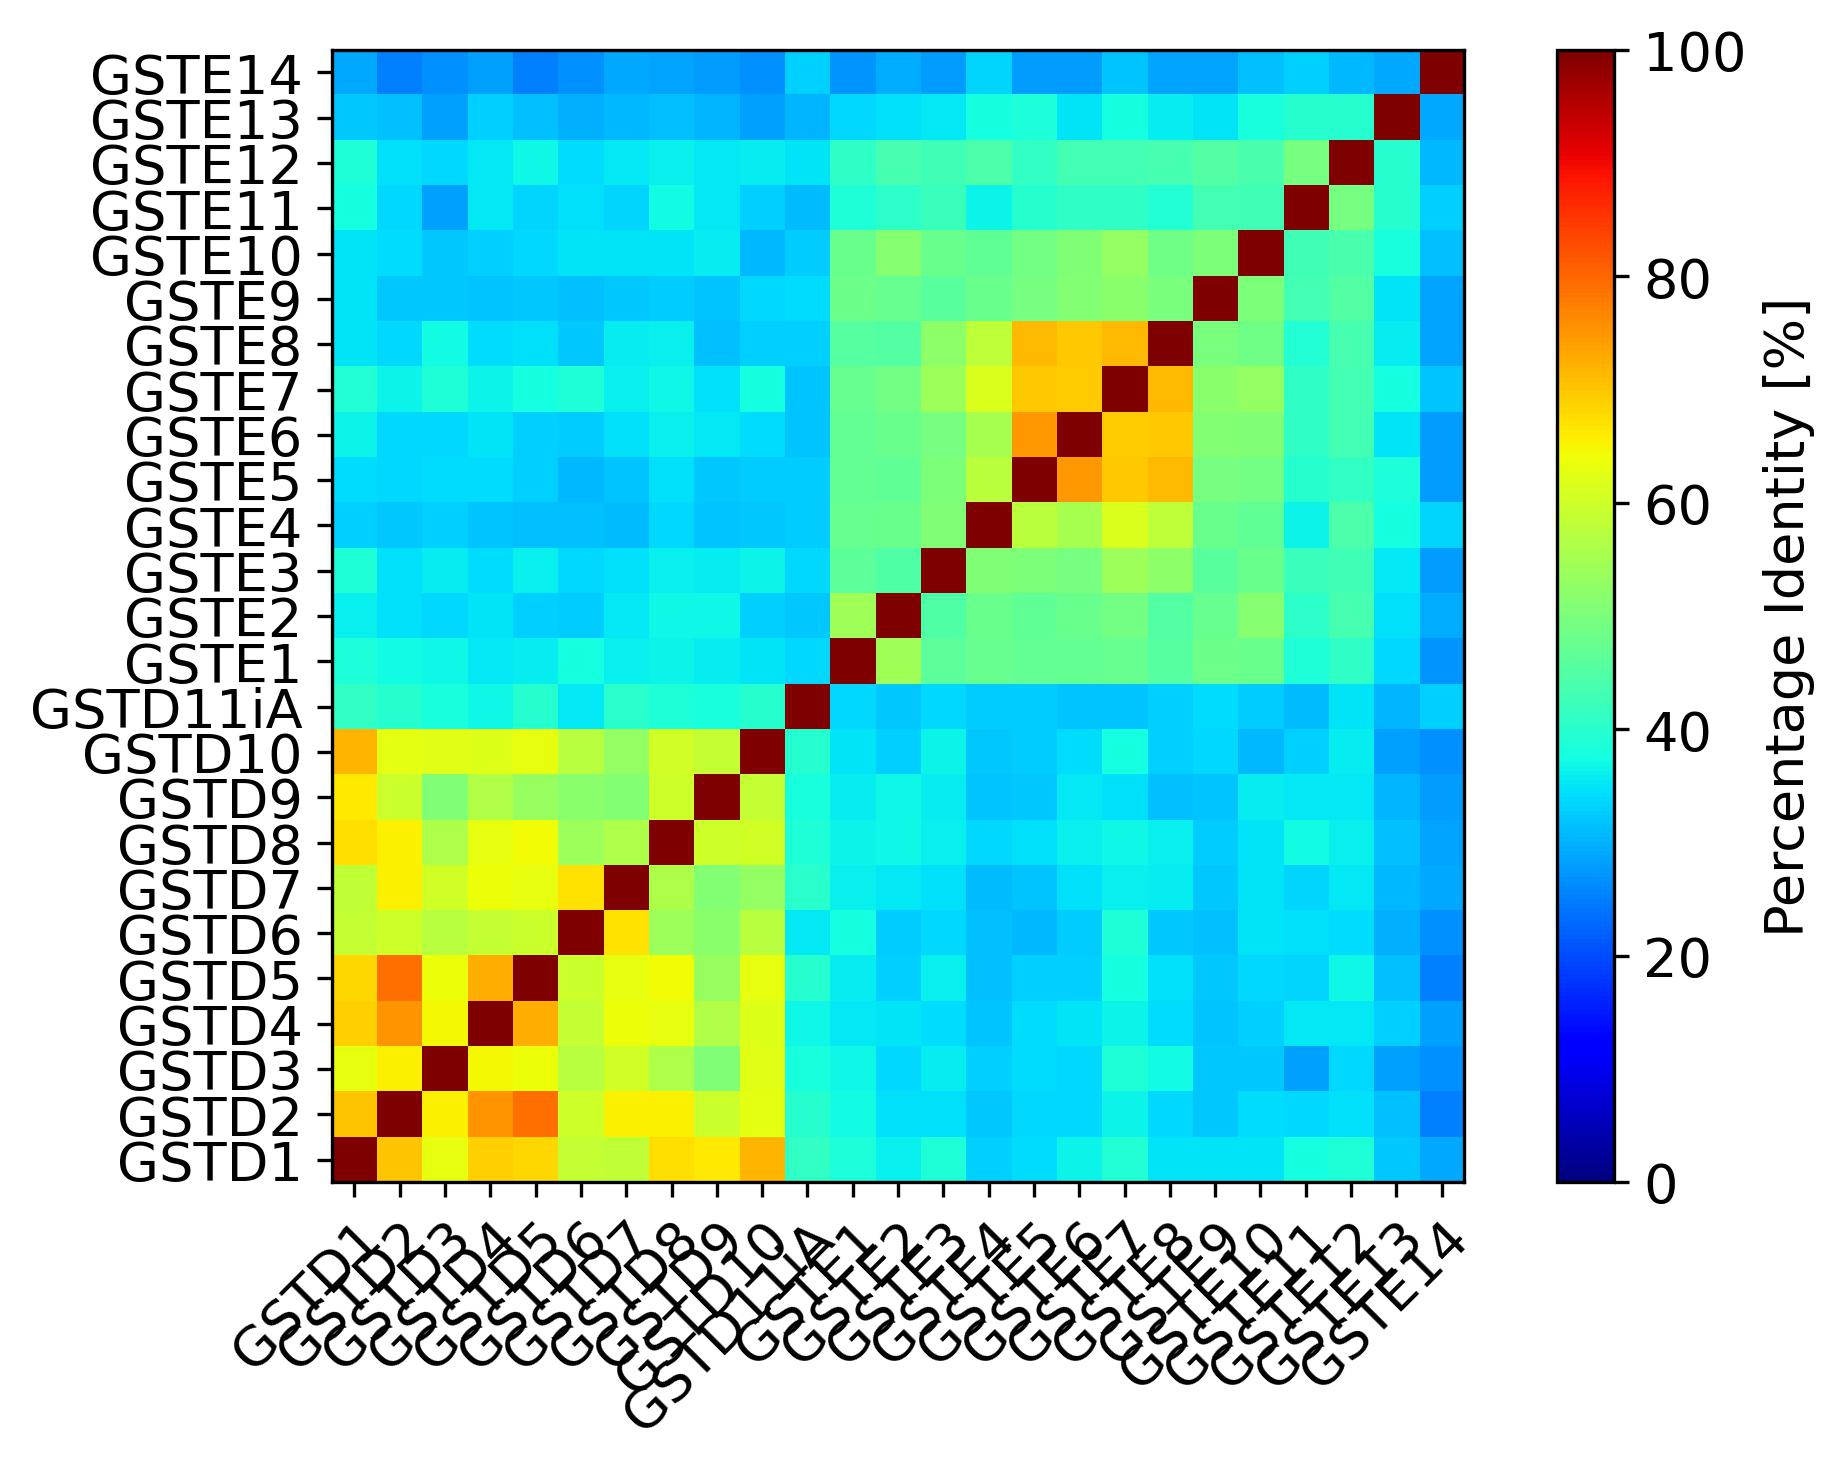
\includegraphics[height = 5cm]{figures/PercentID_matrix.jpg} % ID matrix
	\end{minipage}
	\begin{minipage}{.32\linewidth}
		\textbf{B}\\
		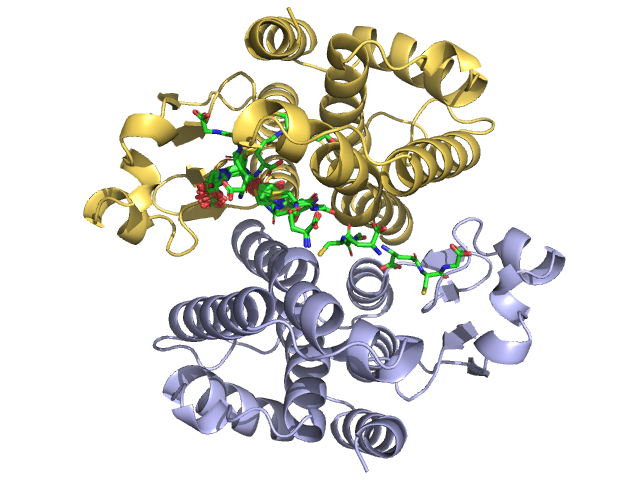
\includegraphics[height = 5cm]{figures/GSTD1_GSHs.png} % 40 positions of GSH		
	\end{minipage}
	\begin{minipage}{.32\linewidth}
		\textbf{C}\\
		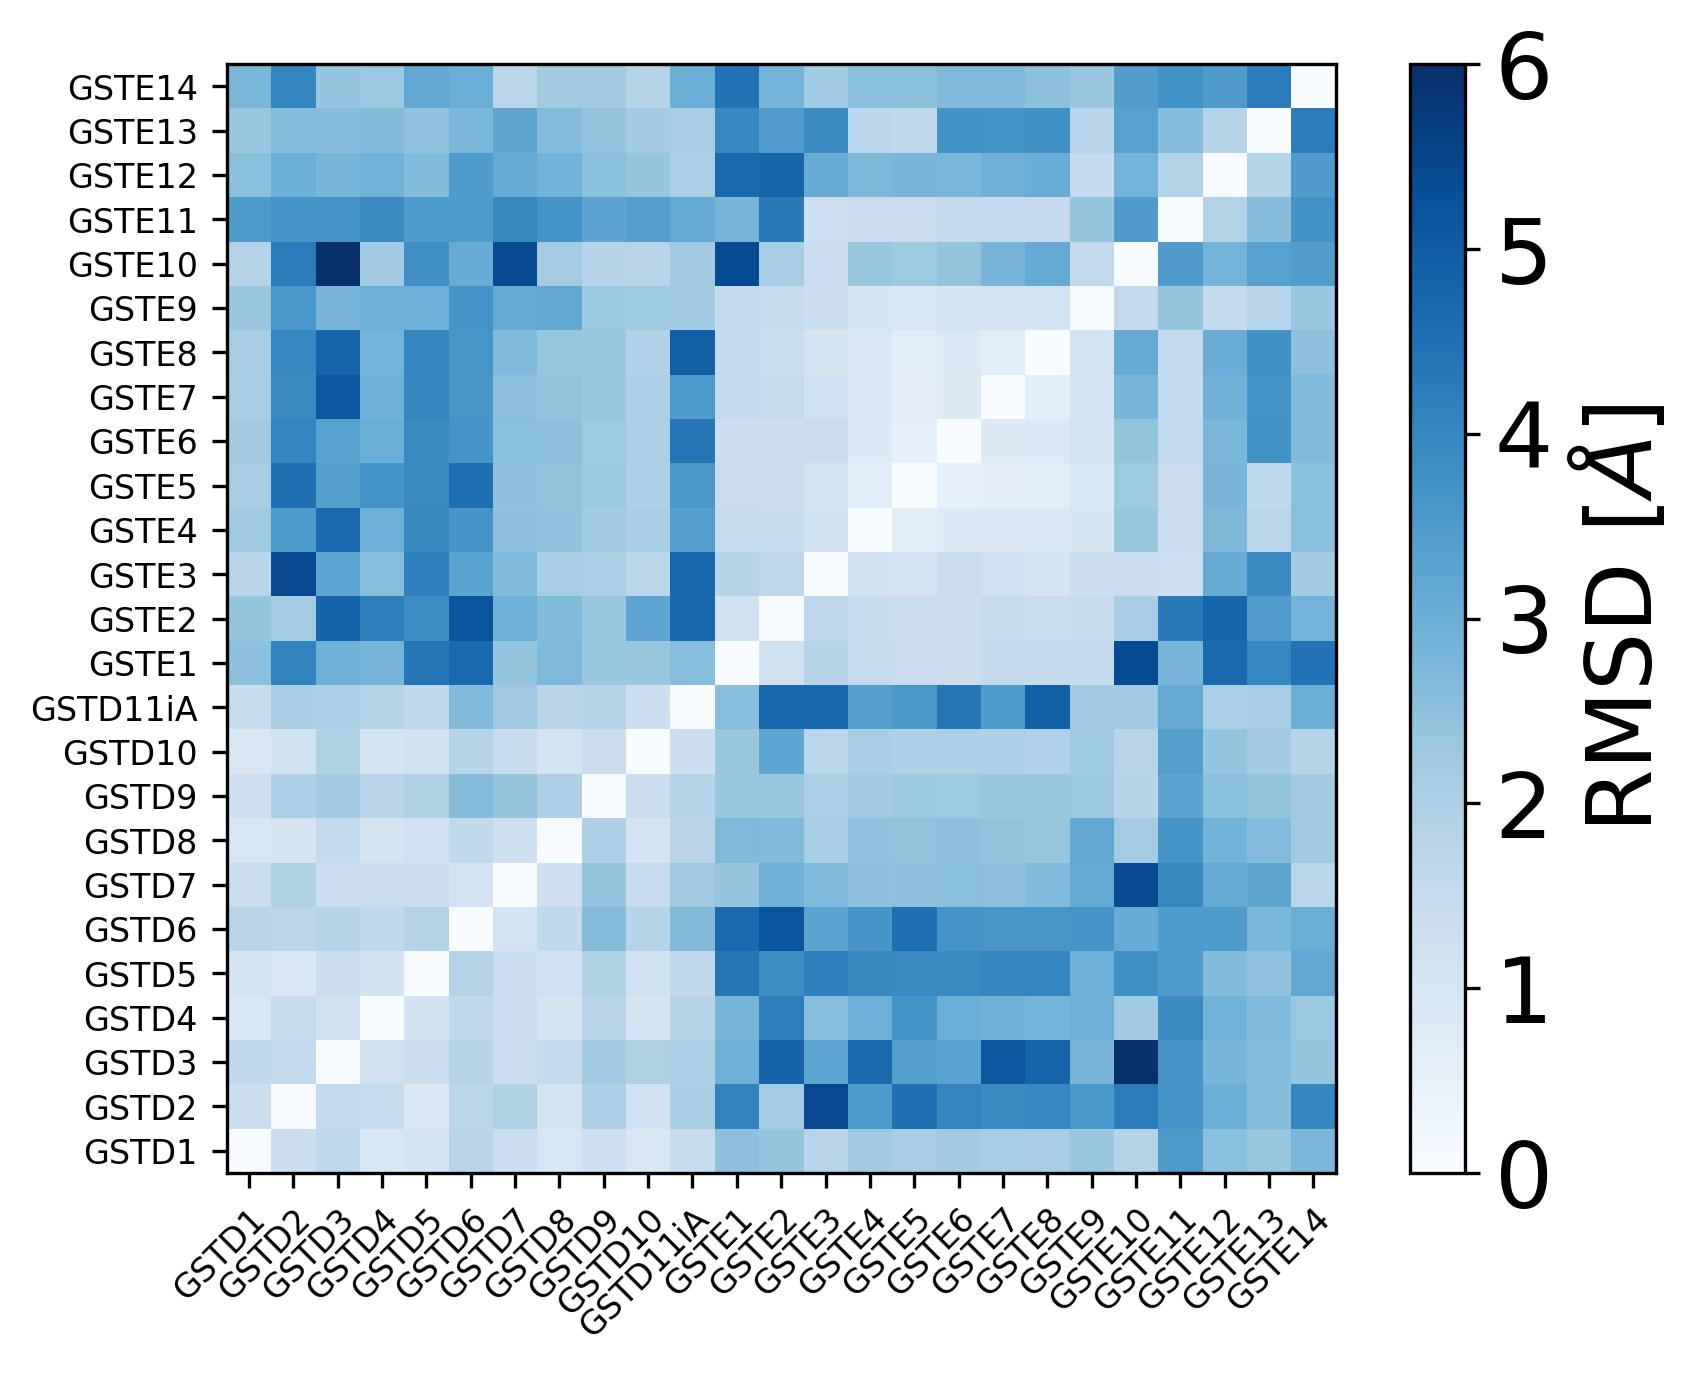
\includegraphics[height = 5cm]{figures/RMSD_matrix.jpg} % RMSD matrix
	\end{minipage}
	\caption{Sequences and structures associated to the selected \textit{Drosophila Melanogaster}'s GSTs}
\end{figure}

\noindent The first step of our methodology was to study the sequences of the GSTs of interest. We computed their Multiple Sequence Alignment as well as the percent identity matrix associated (see Fig. \ref{Sequence & Structure} pannel A). This allows to identify regions of high/low conservation as well as clusters of identity. For instance, it is clearly visible that among the class $\delta$, the GSTs are self similar from a sequence point of view. In contradiction, it seems that among the class $\varepsilon$, the GSTs E5, E6, E7, E8 are self similar but the other ones seems much more different. The sequences were then used as a base for the AlphaFold program to predict the 3D structure (pannel B) and pairs of structures were compared using the Root Mean Squared Deviation (i.e. geometrical distances between atoms, pannel C) and once again in the associated matrix, one can identify two main clusters for class $\delta$ and $\varepsilon$ but here the E10 gives much higher values than we might have expect. This is due to a much longer sequence in the terminal part that make the RMSD higher.

\noindent The information about the structures can be completed by an information about the position of the Glutathione. As mantioned earlier, the program AlphaFill allows to make such precisions and this gives $40$ different positions of Glutathion-like ligands in the GSTD1 (i.e. ligands that are chemically close to Glutathione), those positions are represented in the 3D structure (pannel B). Distances between atoms allowed us to determine from these data the residues that are involved in the protein-ligand binding as well as the dimerization of the structure. Indeed, two atoms that are closer than $3$\AA ~were considered as in contact. This information can be computed for all 25 structures and projected on the MSA matrix computed before. This gives the following representation (see Fig. \ref{MSA + AF + AFi}), where we computed the probability of a given residue to be in the binding site or in the interface of dimerization. From this information, we are able to compute the conservation of any residue in the binding site / interface of dimerization. Here, we give an illustration in the case of the residue $124$, which have a high degree of conservation among all the studied GSTs and have been identified as a part of the binding site in $\%$.

\begin{figure}[h!]
	\label{MSA + AF + AFi}
	\raggedright\textbf{A}
	
\includegraphics[width = .99\linewidth]{figures/MSA_matrix.pdf}\\[.5cm] % MSA + AF + AFi
	\begin{minipage}{.75\linewidth}
		\textbf{B}\\
		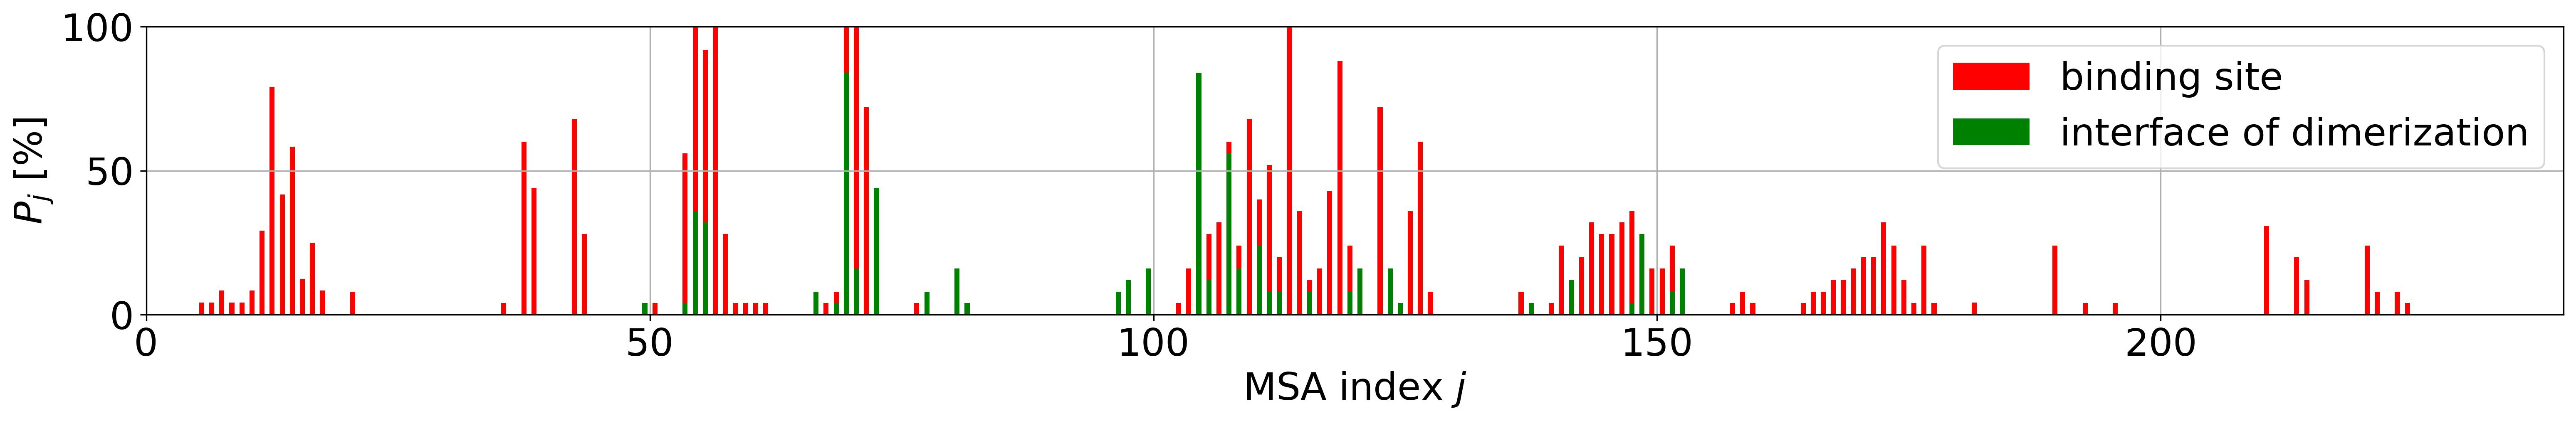
\includegraphics[height = 2cm]{figures/MSA_Proba.jpg} 
	\end{minipage}
	\begin{minipage}{.22\linewidth}
		\textbf{C}\\
		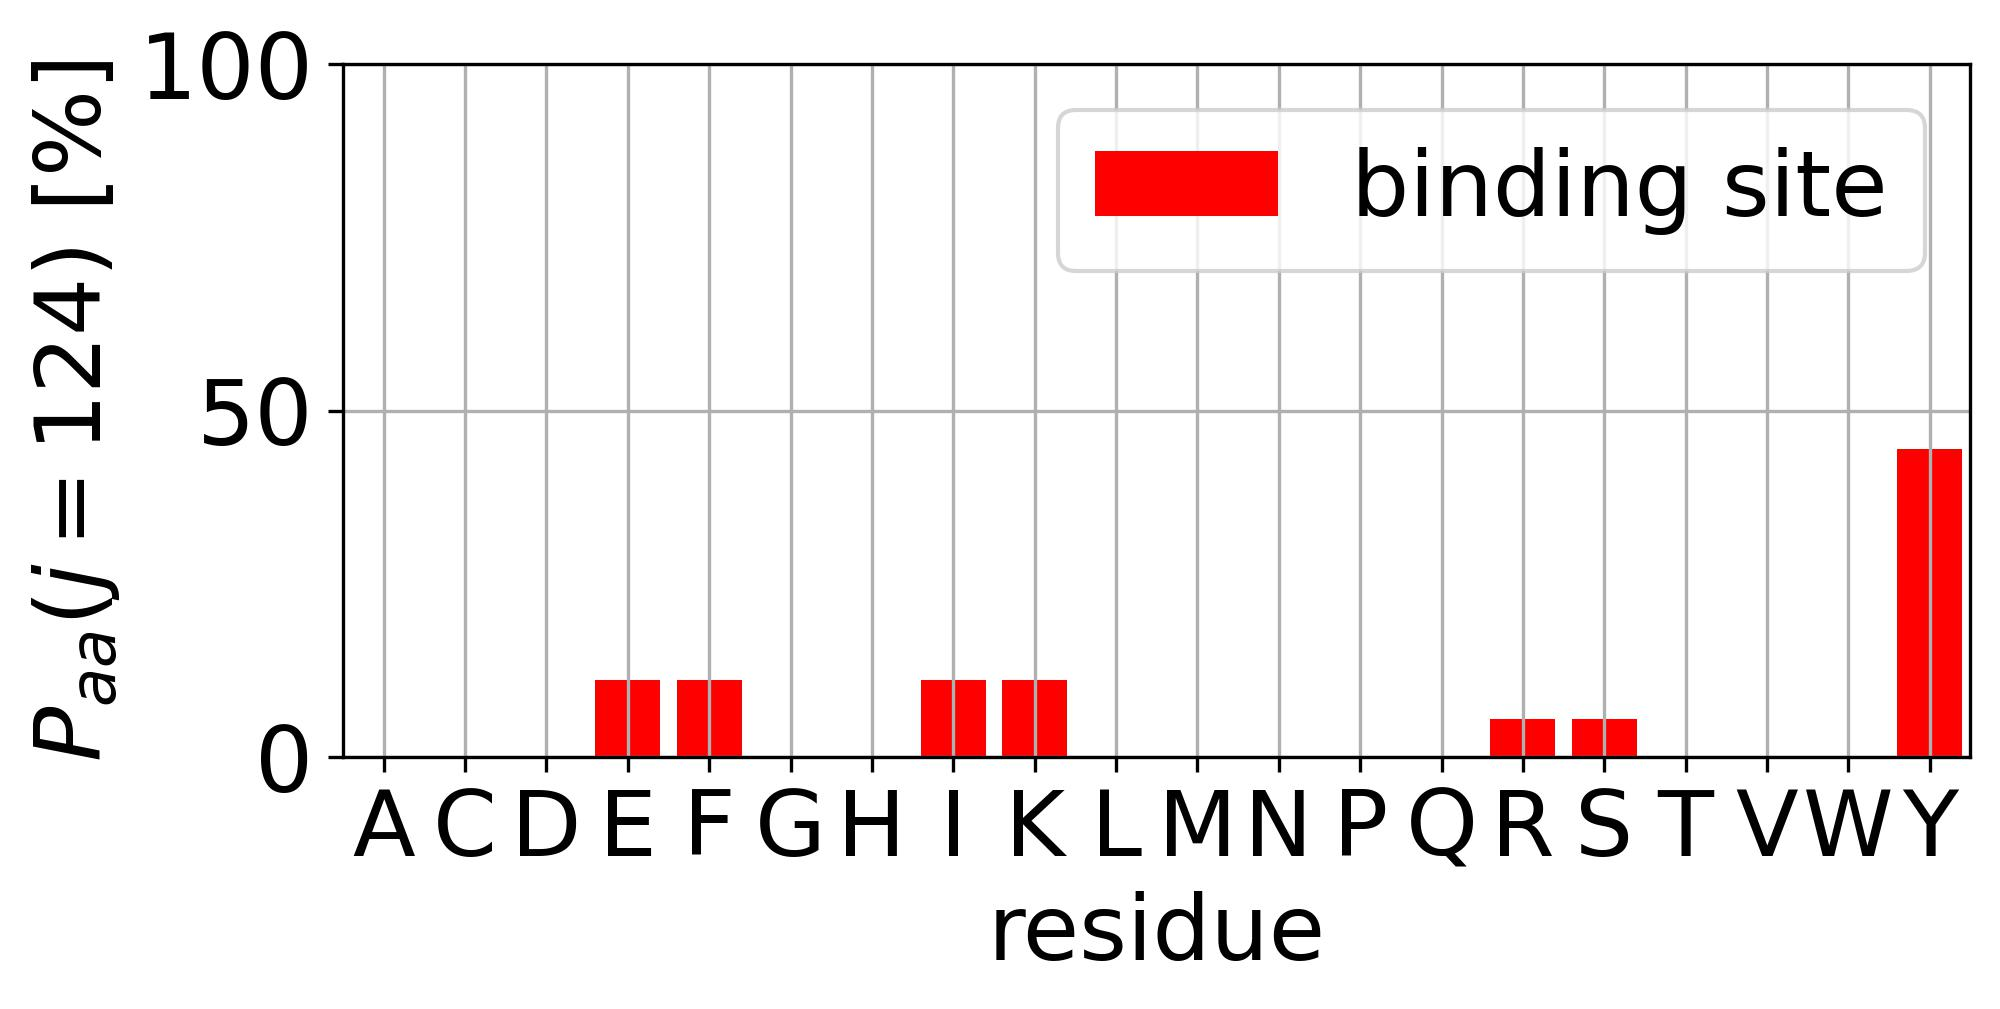
\includegraphics[height = 2cm]{figures/amino-acid_conservation_BS_j=124.jpg} 
	\end{minipage}
	\caption{Indentification of residues in the binding site and of the interface of dimerization}
\end{figure}
   

\section{Dynamics from Normal Modes}
\noindent As explained in the introduction, this present work not only cares about the informations that have been extracted from the static predictions of the AlphaFold and AlphaFill programs but also about the dynamics of the dimers. In this section we will present the next step of our methodology with the Anisotropic Network Model, starting with the parametrization.

\subsection{Parametrization}
\noindent The parametrization step is needed to make sure that the predictions of the model are physically relevant. From the amino-acid's center of mass, it is very simple to compute the mass-weighted Hessian (see eq. \ref{mass-weighted hessian matrix}). As presented before, a first step is to make sure that the cut-off $R_c$ is such that the eigenvalues of the Hessian are non-null. Taking the exemple of the GSTD1, we computed $\tilde{\omega}_k^2 (R_c)$ for the modes $5$, $6$, $7$ and $8$. 

\begin{figure}[h!]
	\label{Rc param}
	\begin{minipage}{.48\linewidth}
		\textbf{A}\\
		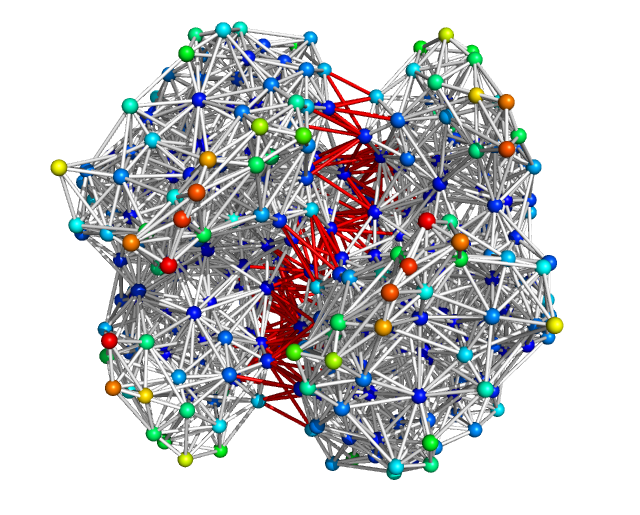
\includegraphics[width = .99\linewidth]{figures/GSTD1_ElasticNetwork.png}
	\end{minipage}	
	\begin{minipage}{.48\linewidth}
		\textbf{B}\\
		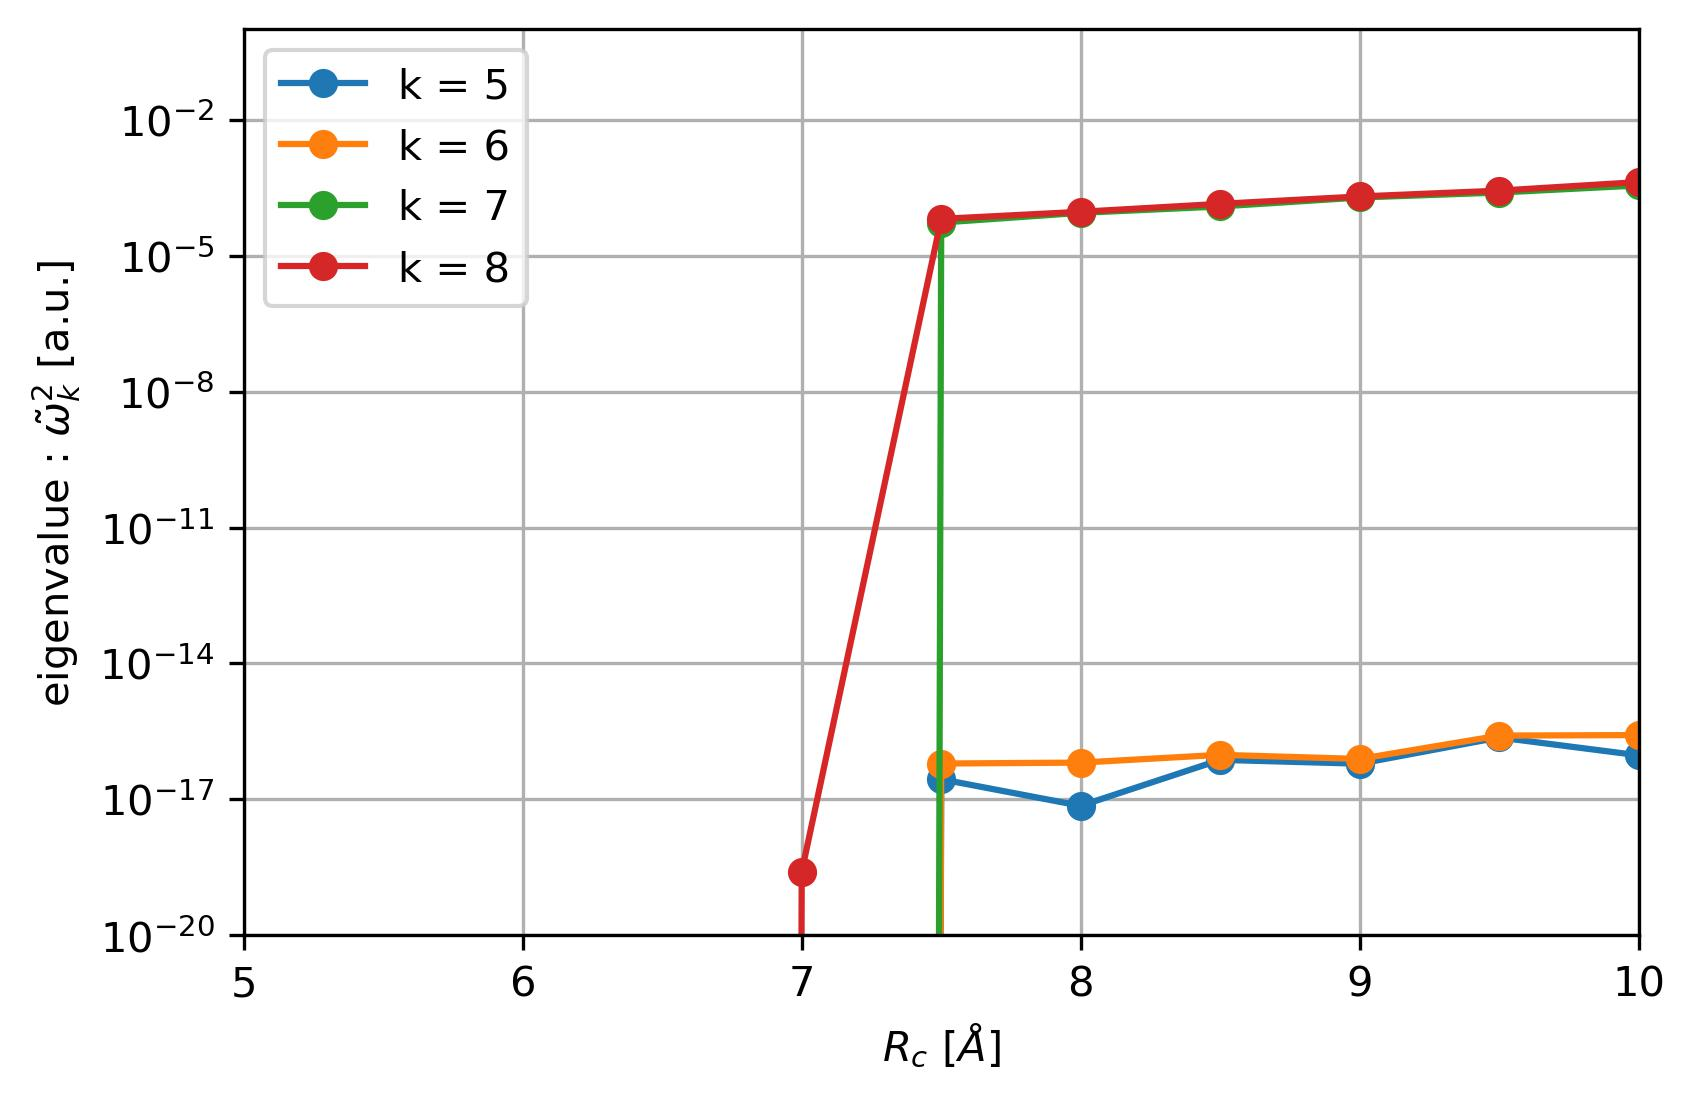
\includegraphics[width = .99\linewidth]{figures/GSTD1_ANM-COM_Rc_param.jpg}\\[.5cm]
	\end{minipage}	
	\caption{Coarse grained representation \& cut-off parametrisation of GSTD1 structure}	
\end{figure}

\noindent In the figure \ref{Rc param}, it is clearly visible that for $R_c = 7.5\AA$, the eigenvalues for $k \ge 6$ are no longer nulls. It is then convenient tu use this value of cut-off for this structure. Note that later, such computations will be performed for all 25 structures in order to have a correct representation of the structures' topology. Those eigenvalues are computed for $\gamma = 1$ kcal.mol$^{-1}$.\AA$^{-2}$, but as we have seen before, $\tilde{\omega}_k^2 \propto \gamma$. It is now time to compute the thermal B-factors to be able to compute the optimal $\gamma$ value.

\subsection{Predictions}
\begin{figure}[h!]
	\label{ANM-COM D1}
	\begin{minipage}{.68\linewidth}
		\textbf{A}\\
		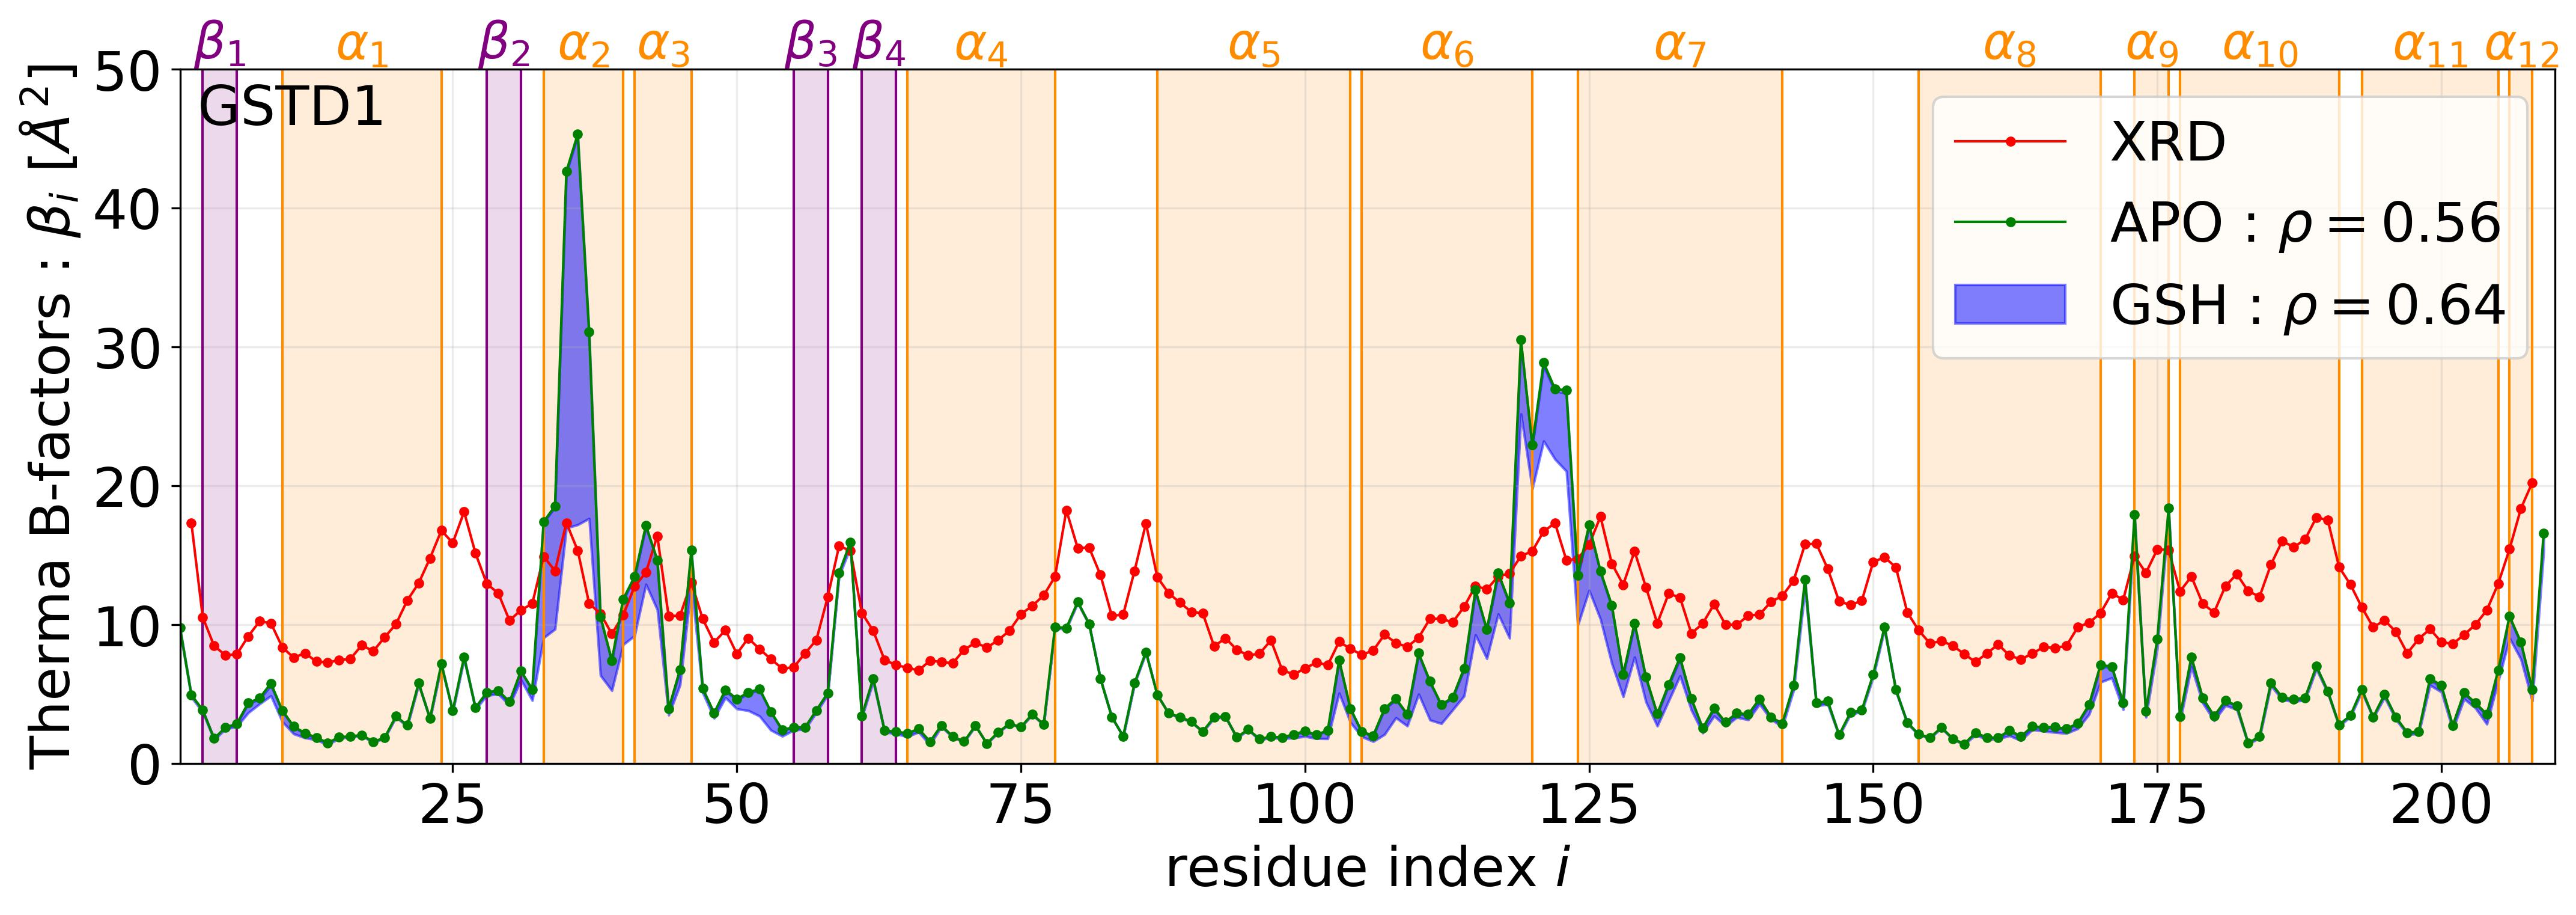
\includegraphics[height = 4cm]{figures/GSTD1+GSH_ANM-COM_Bfactors.jpg}
	\end{minipage}
	\begin{minipage}{.30\linewidth}
		\textbf{B}\\
		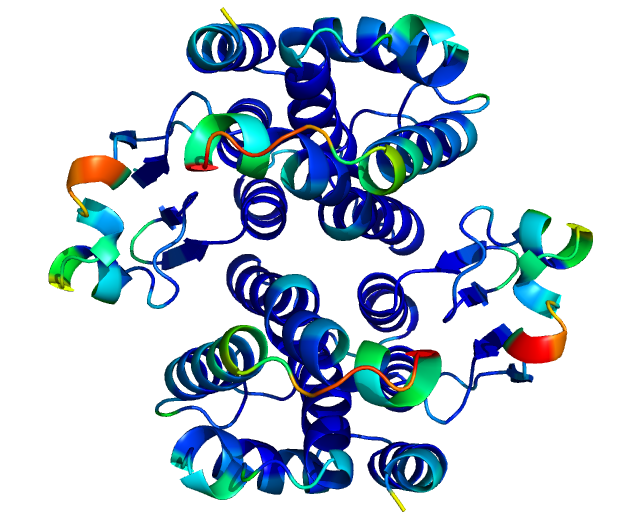
\includegraphics[height = 4cm]{figures/GSTD1_ANM-COM_Bfactors_structure.png}
	\end{minipage}
	\caption{Thermal B-factors predicted from ANM-COM and comparisions with XRD measurments}
\end{figure}

\section{Dynamics from Molecular Dynamics}

\section{Comparison between Structures}
	\chapter{Conclusions and Perspectives}

text here
	\cleardoublepage% le corps du document est terminé
	%
	\appendix
	\pagestyle{back}
	\chapter*{Supporting Information}

\makeatletter
\renewcommand{\fnum@figure}{\figurename~S\thefigure}
\makeatother

\makeatletter
\renewcommand{\fnum@table}{\tablename~S\thetable}
\makeatother

\setcounter{figure}{0}

% MSA Matrix :
\begin{figure}[H]
	\label{MSA + AF + AFi}
	\center
\includegraphics[width = .99\linewidth]{figures/MSA_matrix.pdf} % MSA + AF + AFi
	\caption{MSA matrix for the 25 considered GSTs with the predicted binding site (red residues) and dimer interface (green residues)}
\end{figure}
	
% Conservation in Binding sites :
\begin{figure}
	\label{Conservation BSs}
	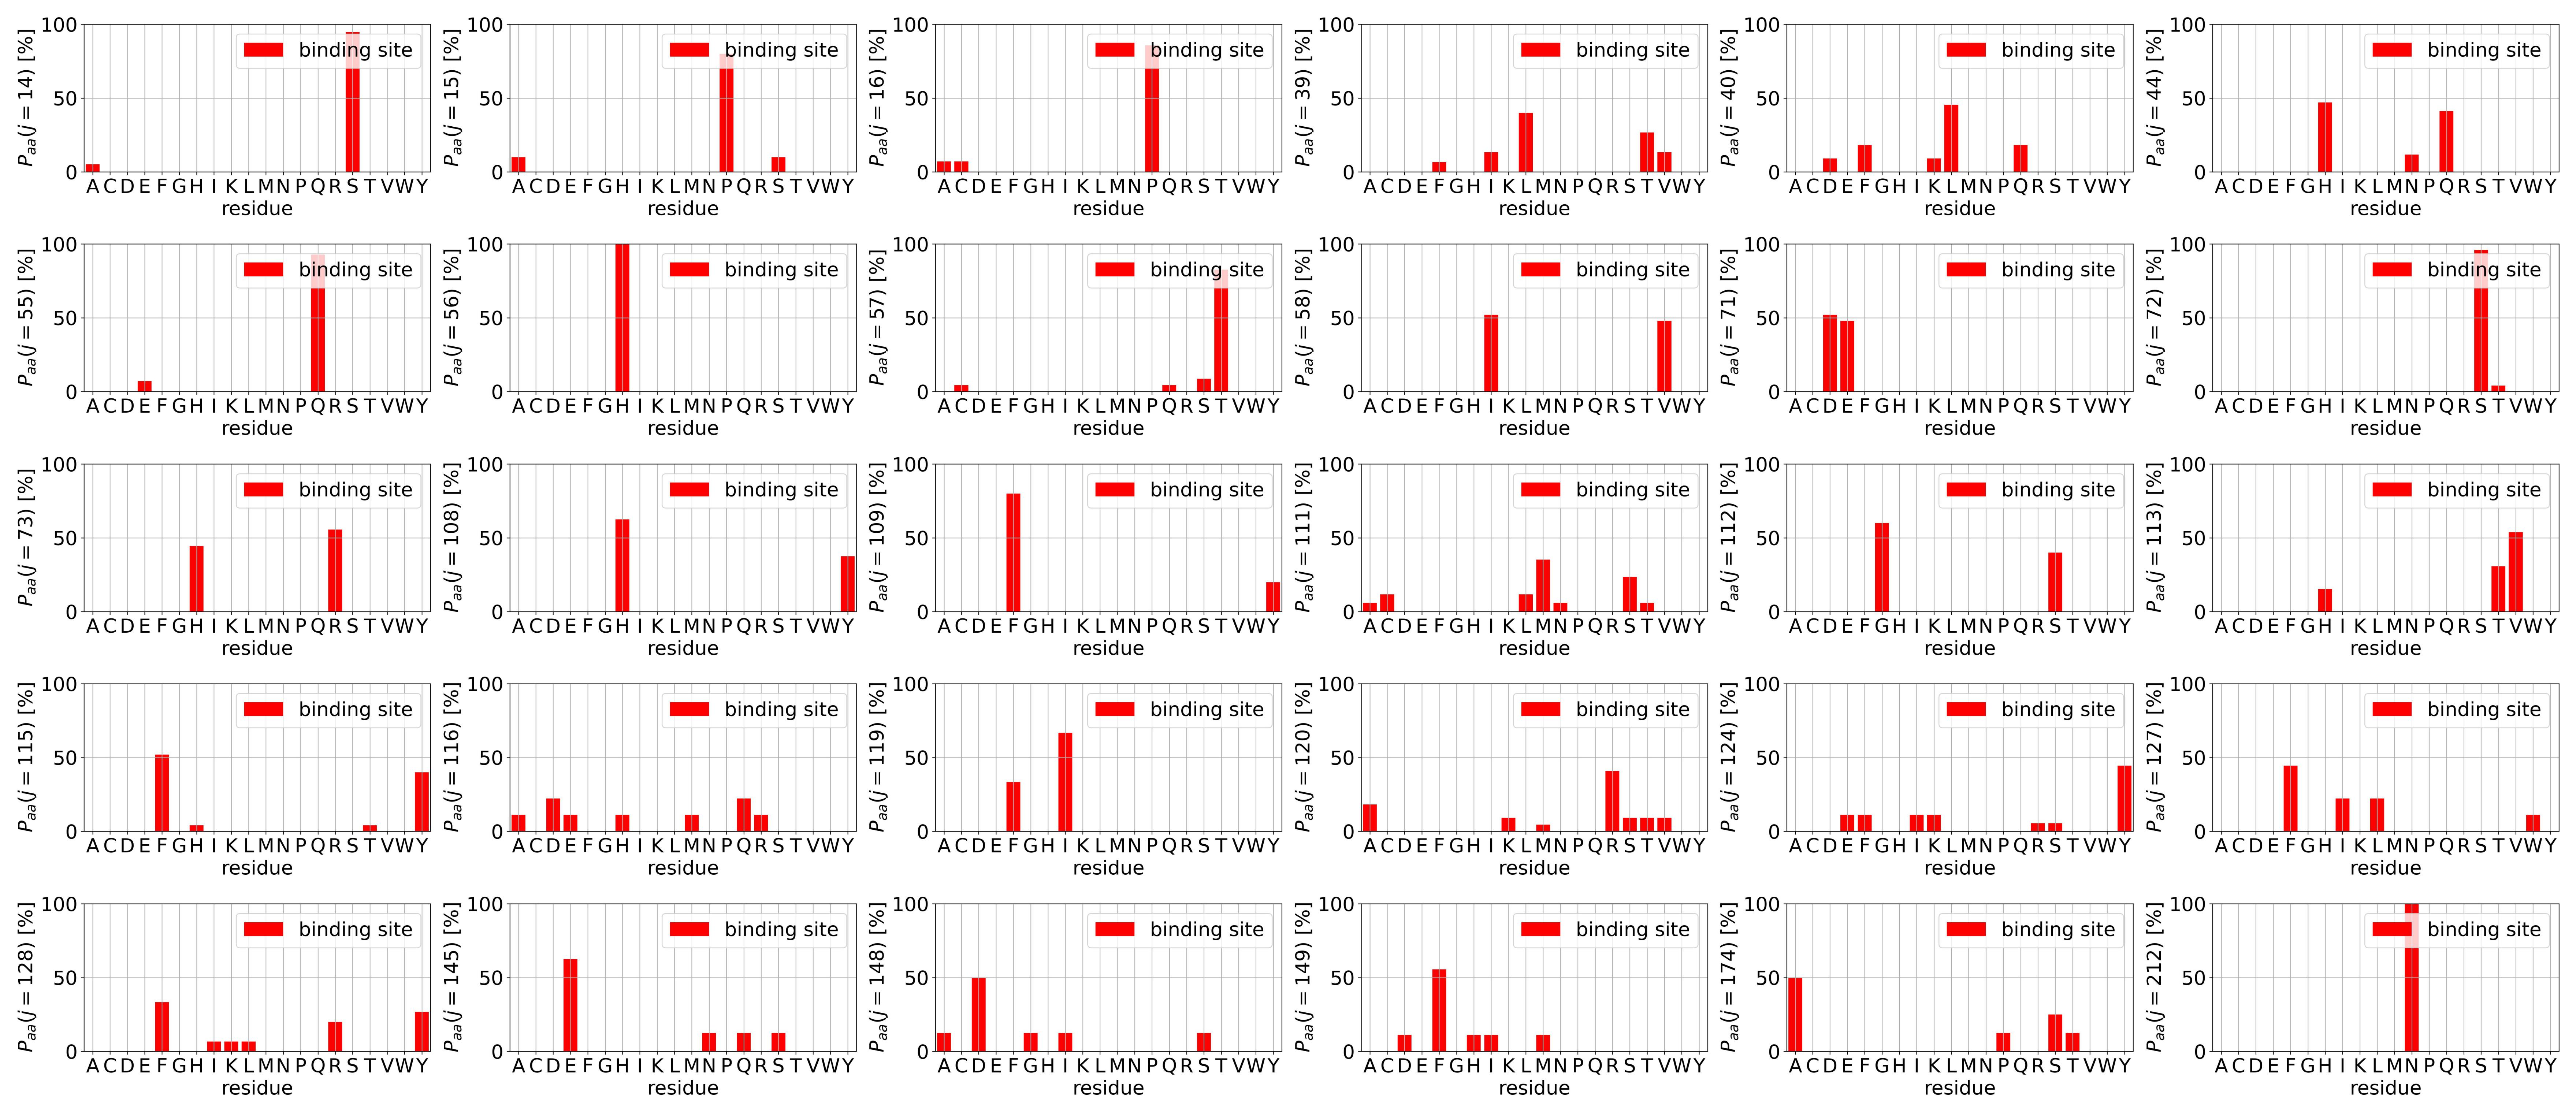
\includegraphics[width = .99\linewidth]{figures/Conservation_array_binding_site.jpg}
	\caption{Conservations of the amino-acids that have been identified as a part of the binding site}
\end{figure}

% Conservation in Dimer interfaces :
\begin{figure}
	\label{Conservation BSs}
	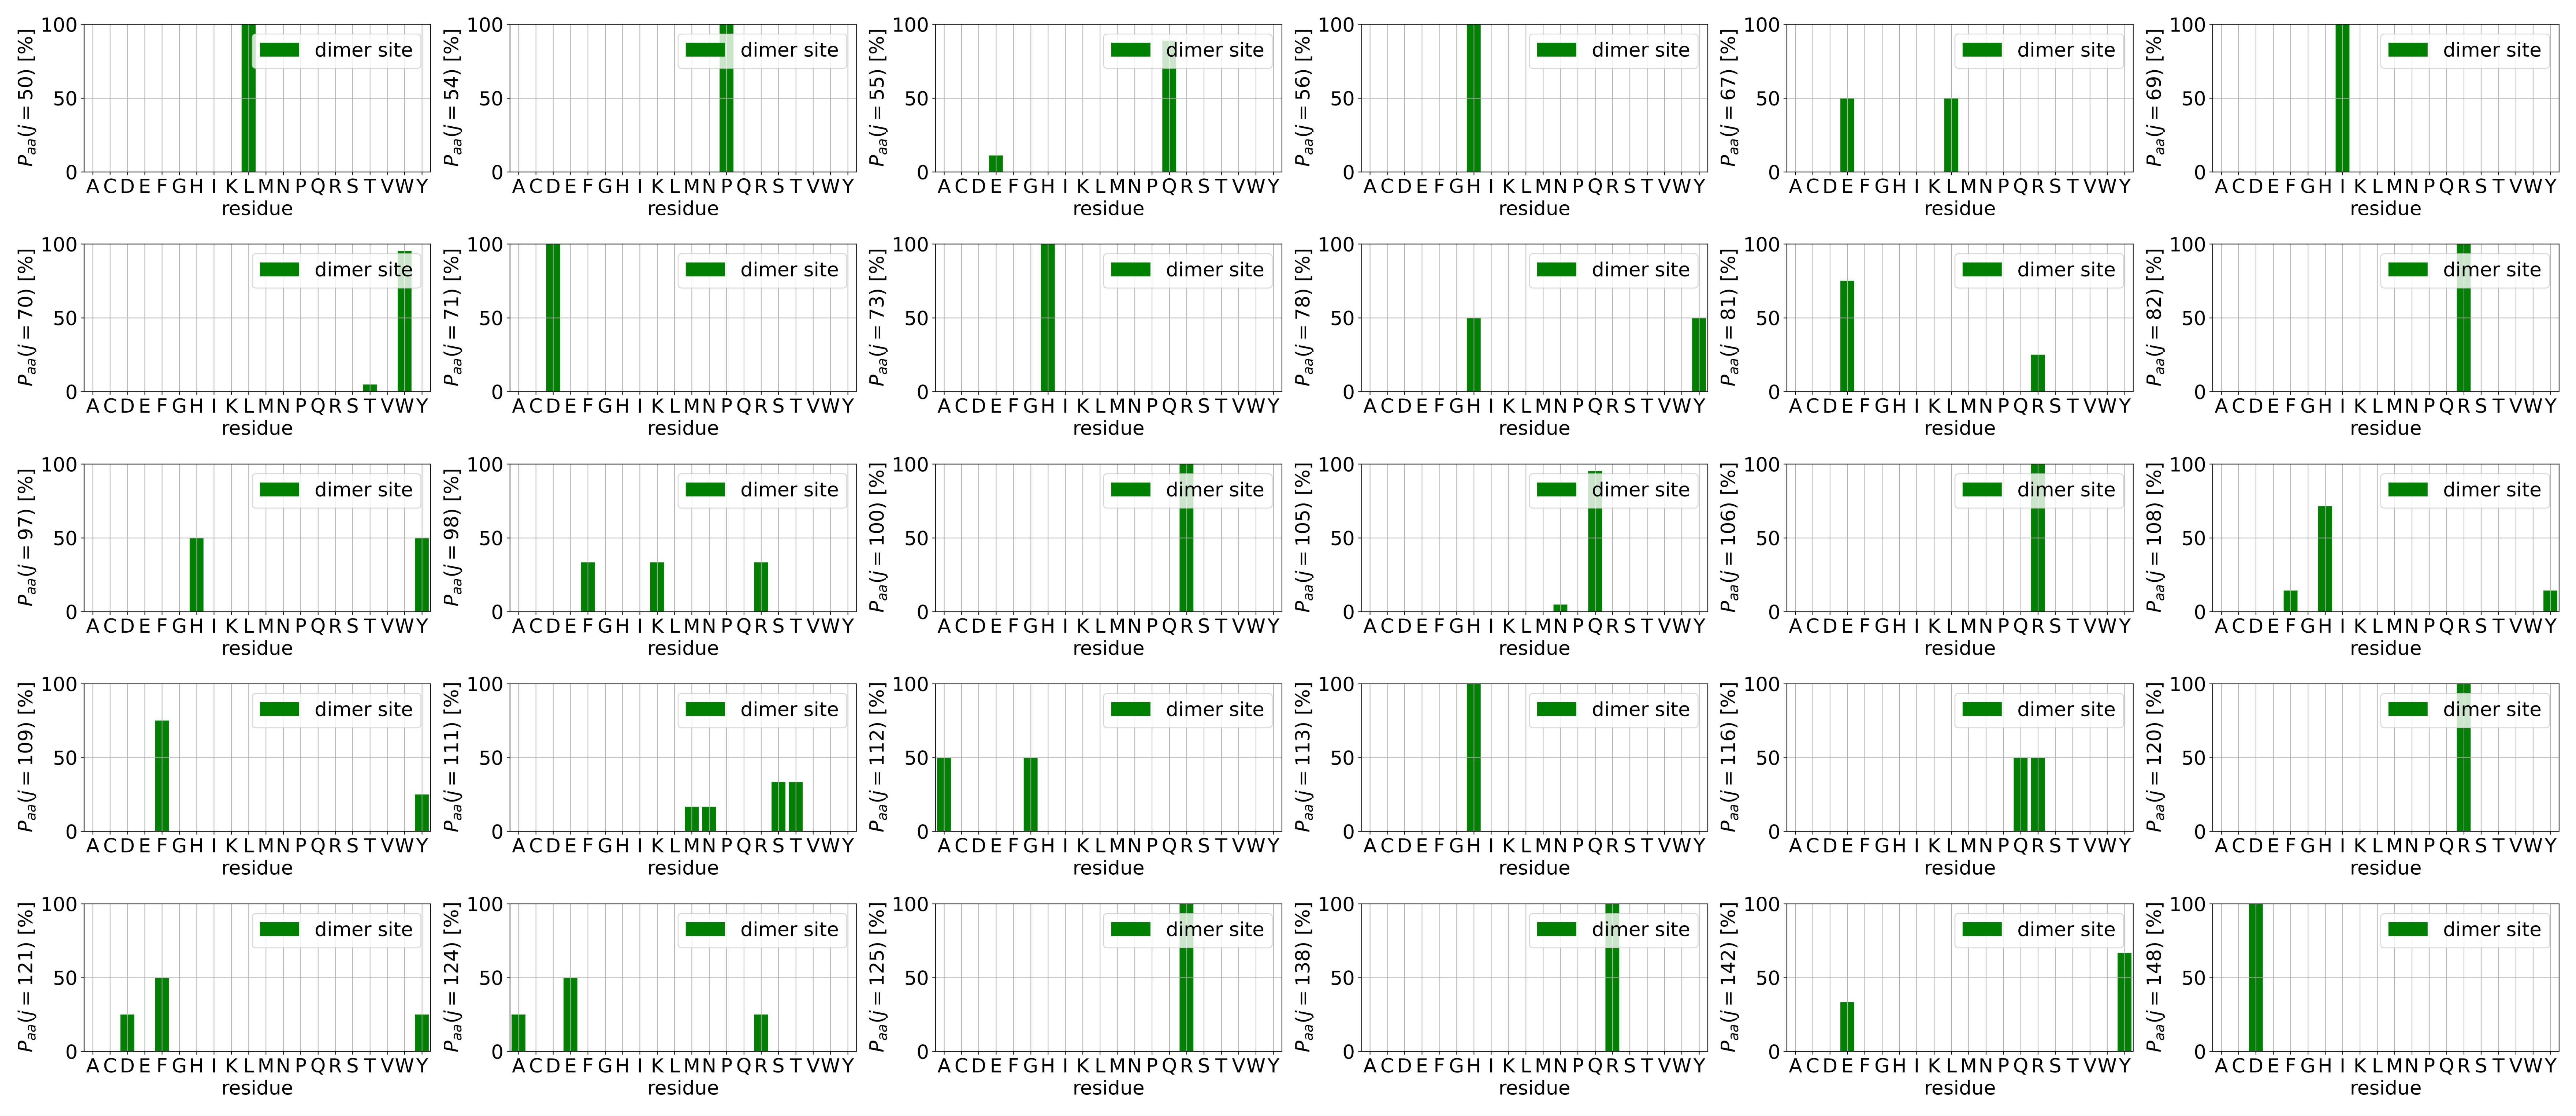
\includegraphics[width = .99\linewidth]{figures/Conservation_array_dimer_interface.jpg}
	\caption{Conservations of the amino-acids that have been identified as a part of the dimer interface}
\end{figure}
	\addcontentsline{toc}{chapter}{Supporting Information}
	\backmatter
	\printbibliography
	\addcontentsline{toc}{chapter}{Bibliography}
	\input{cover_page/back}
	
\end{document}
